\documentclass[a4paper,12pt]{article}

\usepackage[utf8]{inputenc}
\usepackage{amsmath, amssymb}
\usepackage{graphicx}
\usepackage{booktabs}
\usepackage{siunitx}
\usepackage{caption}
\usepackage{subcaption}
\usepackage{geometry}
\usepackage{float}

\geometry{margin=2.5cm}

\graphicspath{{../../graphics}{../../graphics/planar_dielectric_waveguide}{../../graphics/rectangular_dielectric_waveguide}{../../graphics/comsol_individual_waveguide}{../../graphics/comsol_coupled_waveguide}}

\title{Análise de Resultados de Experimentos}
\author{Eduardo A. V. Souza, RA:250950}
\date{\today}

\begin{document}

\maketitle

\section{Semi-analytical analysis}
\label{sec:semi_analytical}

Let's begin the pre-analysis for solving the problem of a beam splitter by studiying some of the materials used in waveguides in the integrated circuit context. The dispersion relation for $Ag_3AsS_3$, $TiO_2$, $Si_3N_4$, and $SiO_2$ are equated in Eq. \ref{eq:ag3ass3_func}, \ref{eq:tio2_func}, \ref{eq:si3n4_func}, \ref{eq:sio2_func}, respectively, and are shown in Fig. \ref{fig:ri_dispersion}. $Ag_3AsS_3$ is used in nonlinear optics: second-harmonic generation, $TiO_2$ is used in high-confinement waveguides in the visible and near-infrared spectrum, $Si_3N_4$ is used in nonlinear optics for supercontinuum generation, and $SiO_2$ is used in optical fibers and planar waveguides.

\begin{subequations}
    \begin{align}
        n_{Ag_3AsS_3} = \sqrt{7.483 + \frac{0.474}{\lambda^2 - 0.09} - 0.0019 \lambda^2}
        \label{eq:ag3ass3_func}
    \end{align}
        
    \begin{align}
        n_{TiO_2} = \sqrt{5.913 + \frac{0.2441}{\lambda^2 - 0.0803}}
        \label{eq:tio2_func}
    \end{align}

    \begin{align}
        n_{Si_3N_4} = \sqrt{1 + \frac{2.8939 \lambda^2}{\lambda^2 - 0.13967^2}}
        \label{eq:si3n4_func}
    \end{align}

    \begin{align}
        n_{SiO_2} = \sqrt{1 + \frac{0.6961663 \lambda^2}{\lambda^2 - 0.0684043^2} + \frac{0.4079426 \lambda^2}{\lambda^2 - 0.1162414^2} + \frac{0.8974794 \lambda^2}{\lambda^2 - 9.896161}}
        \label{eq:sio2_func}
    \end{align}
\end{subequations}

Figure \ref{fig:critical_angle} shows the critical angle as a function of the cladding refractive index for the core made of the materials stated above. You can see that as we increase the cladding RI (refractive index), the modes become more leaky and the critical angle increases, being easier to couple light in the waveguide. In the opposite direction, as we increase the core RI, the modes become more confined and the critical angle decreases, being harder to couple light in the waveguide.

\begin{figure}[H]
    \centering
    \begin{subfigure}{0.45\textwidth}
        \centering
        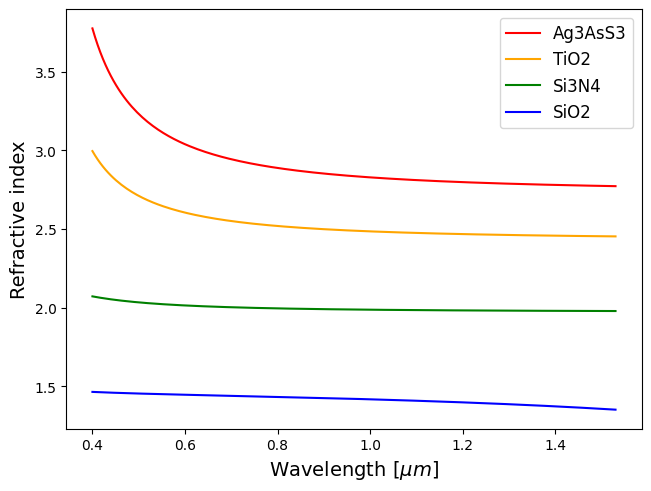
\includegraphics[scale=0.45]{dispersion_relation.png}
        \caption{Dispersion relation.}
        \label{fig:ri_dispersion}
    \end{subfigure}
    \hfill
    \begin{subfigure}{0.45\textwidth}
        \centering
        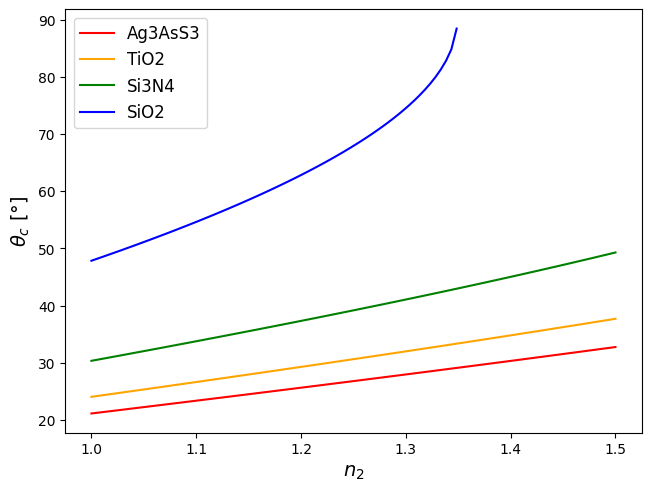
\includegraphics[scale=0.45]{critical_angle_vs_refractive_index.png}
        \caption{Critical angle.}
        \label{fig:critical_angle}
    \end{subfigure}
    \caption{Study of different materials for the core of the waveguide.}
\end{figure}

\subsection{Planar dielectric waveguide}
\label{subsec:planar_dielectric_waveguide}

A important parameter for waveguides is the numerical aperture ($NA$), which is a measure of the light acceptance angle in the waveguide. It is given by Eq. \ref{eq:NA}, where $n_1$ is the refractive index of the core and $n_2$ is the refractive index of the cladding. 

\begin{equation}
    NA = \sqrt{n_1^2 - n_2^2} 
    \label{eq:NA}
\end{equation}

The other important parameter is the critical angle ($\theta_c$), given by Eq. \ref{eq:theta_c}, related to the maximum angle of incidence for total internal reflection to occur.

\begin{equation}
    \theta_c = \sin^{-1} \left(\frac{n_2}{n_1}\right) 
    \label{eq:theta_c}
\end{equation}

The results for these parameters for $SiO_2$ and $TiO_2$ are shown in Tab. \ref{tab:na_theta_c}.

\begin{table}[H]
    \centering
    \begin{tabular}{ccc}
        \toprule
        Material & $\theta_c [^\circ]$ & $NA$ \\
        \midrule
        $SiO_2$ & 47.8 & 0.906 \\
        $TiO_2$ & 24.1 & 2.240 \\
        \bottomrule
    \end{tabular}
    \caption{Numerical aperture and critical angle for different core materials, considering air as the cladding.}
    \label{tab:na_theta_c}
\end{table}

A approximation for the number of TE modes is given by \eqref{eq:number_of_modes_approx}, where $d$ is the core thickness, $\lambda$ is the wavelength, and $NA$ is the numerical aperture. 

\begin{equation}
    M_{the} \doteq 2 \frac{d}{\lambda} NA
    \label{eq:number_of_modes_approx}
\end{equation}

The exact number of modes can be found by solving the characteristic equation for the planar dielectric waveguide, given by Eq. \ref{eq:char_eq}, where $m = 0, 1, 2, ...$ is the mode order, $k_0 = 2 \pi / \lambda$ is the free space wavenumber, $\theta_m$ is the angle of incidence for the m-th mode, and $\theta_c$ is the critical angle.

\begin{equation}
    f_1(\sin(\theta_m)) \equiv \tan\left[ \pi \left(\frac{\sin(\theta_m) d}{\lambda} - \frac{m}{2}\right) \right] =
    \sqrt{\frac{\sin^2(\overline{\theta}_c)}{\sin(\theta_m)^2} - 1}
    \label{eq:char_eq} \equiv f_2(\sin(\theta_m))
\end{equation}

The plot for $f_1$ and $f_2$ to help visualize the possible modes for the waveguide is shown in Fig. \ref{fig:char_eq}. Using the bisection or the Newton-Raphson methods based on the guess interval or point aided by Fig. \ref{fig:char_eq}, we can find the intersections of $f_1$ and $f_2$ to further calculate the propagation constant $\beta_m$ and the effective RI (ERI) $n_{eff,m}$ for the m-th order mode. The resultant modes are shown in Fig. \ref{fig:shell_modes} where the black dots are the modes, the green curve have radius $n_2 k_0$ and the blue curve have radius $n_2 k_0$. For a planal dielectric waveguide with $SiO_2$ as the core and with thickness $d = 10\mu$ we got 5 possible TE modes.

\begin{figure}[H]
    \centering
    \begin{subfigure}{0.45\textwidth}
        \centering
        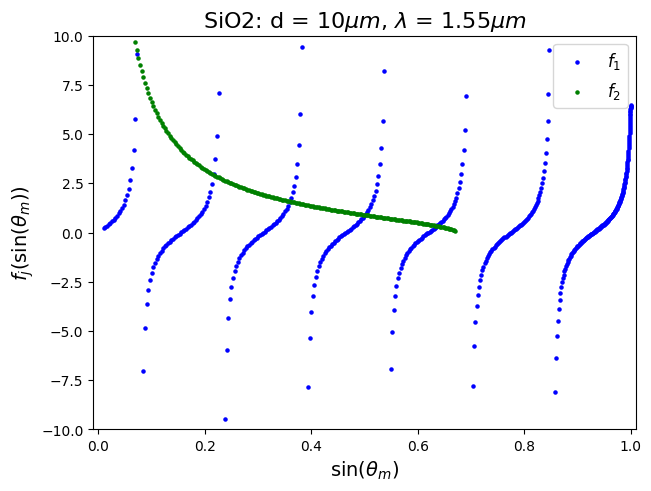
\includegraphics[scale=0.45]{modes_SiO2_d10um_wv1.55um.png}
        \caption{Characteristic equation.}
        \label{fig:char_eq}
    \end{subfigure}
    \hfill
    \begin{subfigure}{0.45\textwidth}
        \centering
        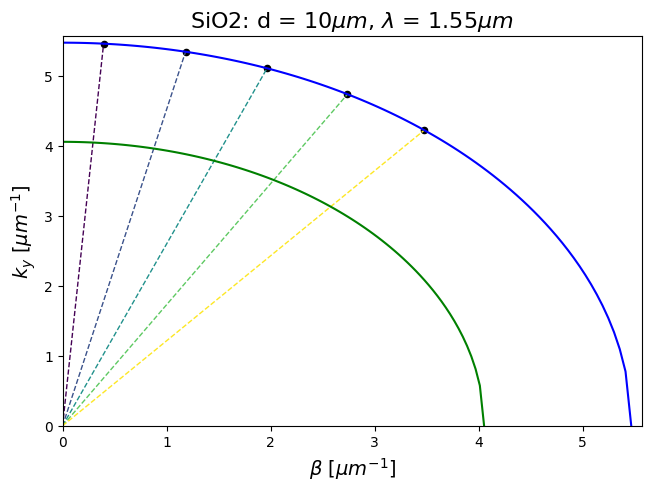
\includegraphics[scale=0.45]{modeshell_SiO2_d10um_wv1.55um.png}
        \caption{Guided modes.}
        \label{fig:shell_modes}
    \end{subfigure}
    \caption{Solution for the guided modes in a planar dielectric waveguide with a $SiO_2$ core, $d = 10 \mu m$ and $\lambda = 1.55 \mu m$.}
\end{figure}

A comparison between the approximation and exact number of TE modes is put in Tab. \ref{tab:number_of_modes_comparison} as we increase the thickness of the core, by consequence, we increase the number of possible modes. So, when it is possible to manually count the number of modes, use this technique to obtain the exact value, since the approximate value can diverge much.

\begin{table}[H]
    \centering
    \begin{tabular}{ccc}
        \toprule
        $d [\mu m]$ & $M_{app}$ & $M_{exa}$ \\
        \midrule
        1 & 2 & 1 \\
        5 & 6 & 3 \\
        10 & 12 & 5 \\
        \bottomrule
    \end{tabular}
    \caption{Approximate and exact number of TE modes for different core thicknesses for the $SiO_2$ waveguide.}
    \label{tab:number_of_modes_comparison}
\end{table}

Using the condition $k_0 n_2 \leq \beta_m \leq k_0 n_1$ to keep only the guided modes, we get the values for the propagation constant and the corresponding ERI for $SiO_2$-core waveguide in Tab. \ref{tab:beta_sio2}. Running the same simulation but for the $TiO_2$-core waveguide, we get the values of Tab. \ref{tab:beta_tio2}.

\begin{table}[H]
    \centering
    \begin{subtable}{0.45\textwidth}
        \centering
        \begin{tabular}{ccc}
            \toprule
            Mode & $\beta [\mu m^{-1}]$ & $n_{eff}$ \\
            \midrule
            0 & 5.419 & 1.337 \\
            1 & 5.008 & 1.235 \\
            2 & 4.171 & 1.029 \\
            \bottomrule
        \end{tabular}
        \caption{$SiO_2$.}
        \label{tab:beta_sio2}
    \end{subtable}
    \hfill
    \begin{subtable}{0.45\textwidth}
        \centering
        \begin{tabular}{ccc}
            \toprule
            Mode & $\beta [\mu m^{-1}]$ & $n_{eff}$ \\
            \midrule
            0 & 9.847 & 2.429 \\
            1 & 9.034 & 2.229 \\
            2 & 7.194 & 1.775 \\
            \bottomrule
        \end{tabular}
        \caption{$TiO_2$.}
        \label{tab:beta_tio2}
    \end{subtable}
    \caption{Propagation constant and effective refractive index in a planar dielectric waveguide with $d = 5 \mu m$ and $\lambda = 1.55 \mu m$.}
\end{table}

As we can see by the results above, the waveguide with core made by $TiO_2$ confines light much more than the one made by $SiO_2$. 

\subsection{Rectangular dielectric waveguide}
\label{subsec:rectangular_dielectric_waveguide}
    
Now, to solve the problem of a rectangular dielectric waveguide, we will use the Marcatili's approximation, that is, we will consider that $E(x, y) = X(x)Y(y)$. In other words, this problem is reduced to two planar dielectric waveguide problems (solved in Sec. \ref{subsec:planar_dielectric_waveguide}).

Let's start with the analysis of the number of modes for the waveguide made of $SiO_2$ with $w = 6\mu m$ and $t = 2\mu m$, for a input light with $\lambda = 1.55\mu m$. The characteristic equation and the diagram with the guided modes are shown in Fig. \ref{fig:char_eq2} and \ref{fig:shell_modes2}, respectively.

\begin{figure}[H]
    \centering
    \begin{subfigure}{0.45\textwidth}
        \centering
        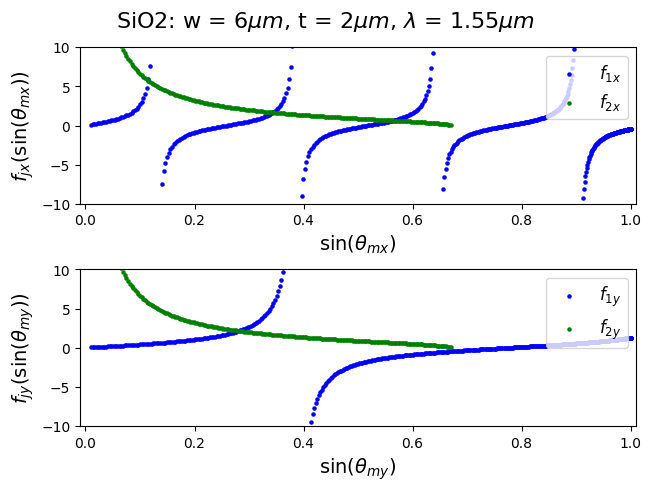
\includegraphics[scale=0.45]{modes_SiO2_w6um_t2um_wv1.55um.png}
        \caption{Characteristic equation.}
        \label{fig:char_eq2}
    \end{subfigure}
    \hfill
    \begin{subfigure}{0.45\textwidth}
        \centering
        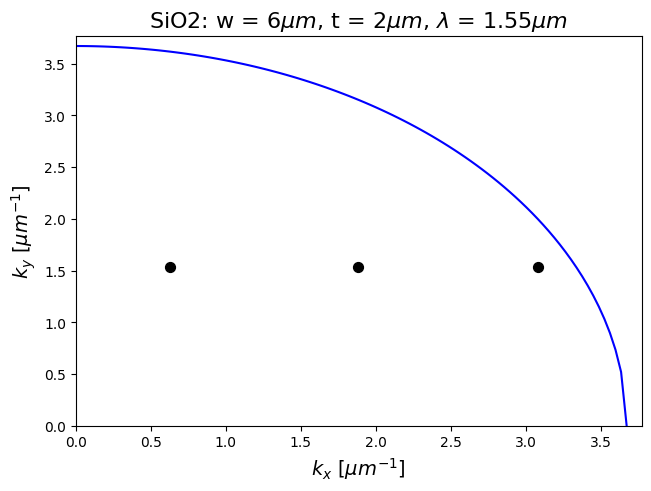
\includegraphics[scale=0.45]{modeshell_SiO2_w6um_t2um_wv1.55um.png}
        \caption{Guided modes.}
        \label{fig:shell_modes2}
    \end{subfigure}
    \caption{Solution for the guided modes in a rectangular dielectric waveguide with a $SiO_2$ core, $w = 6 \mu m$, $t = 2\mu m$, and $\lambda = 1.55 \mu m$.}
\end{figure}

The propagation constant and the refractive index for the guided modes are organized in Tab. \ref{tab:beta_sio2} for $SiO_2$ and in Tab. \ref{tab:beta_tio2} for $TiO_2$.

\begin{table}[H]
    \centering
    \begin{subtable}{0.45\textwidth}
        \centering
        \begin{tabular}{ccc}
            \toprule
            Mode & $\beta [\mu m^{-1}]$ & $n_{eff}$ \\
            \midrule
            (0,0) & 5.211 & 1.285 \\
            (1,0) & 4.901 & 1.209 \\
            (2,0) & 4.247 & 1.048 \\
            \bottomrule
        \end{tabular}
        \caption{$SiO_2$.}
    \end{subtable}
    \hfill
    \begin{subtable}{0.45\textwidth}
        \centering
        \begin{tabular}{ccc}
            \toprule
            Mode & $\beta [\mu m^{-1}]$ & $n_{eff}$ \\
            \midrule
            (0,0) & 9.401 & 2.319 \\
            (1,0) & 8.793 & 2.169 \\
            (2,0) & 7.453 & 1.839 \\
            (3,0) & 4.928 & 1.216 \\
            \bottomrule
        \end{tabular}
        \caption{$TiO_2$.}
        \label{tab:modes_d5um}
    \end{subtable}
    \caption{Propagation constant and effective refractive index in a rectangular dielectric waveguide with $w = 6 \mu m$, $t = 3\mu m$, and $\lambda = 1.55 \mu m$.}
\end{table}

As you can see by the results above, further from confining more the light inside the core, the $TiO_2$ waveguide also present one more mode than the $SiO_2$ waveguide for the same width and thickness parameters.

\section{COMSOL analysis}
\label{sec:comsol}

\subsection{Individual guides}
\label{subsec:individual_guides}

Now, let's model the rectangular dielectric waveguide in COMSOL Multiphysics and compare the results with those obtained using the Marcatili's method. Consider from now on the cladding material to be air ($n_2 = 1.000$), the input wavelength to be $\lambda = 1.55 \mu m$, the core width to be $w = 6 \mu m$ and the core thickness to be $t = 2 \mu m$.

Given the dispersion relation you can calculate the relative permittivity by Eq. \eqref{eq:eps_r}.

\begin{equation}
    \epsilon_r(\lambda) = \frac{n(\lambda)^2}{\mu_r(\lambda)}
    \label{eq:eps_r}
\end{equation}

Also, consider the following parameters for the first simulation:
\begin{itemize}
    \item Core material: $SiO_2$.
    \item Dispersion relation: Eq. \eqref{eq:sio2_func}.
    \item Relative permeability: 1.
    \item Electric condutivity: $\sigma = 1 \cdot 10^{12}S/m$.
\end{itemize}

I ran the simulation for the first six modes, obtained the effective refractive index and calculated the propagation constant by $\beta = n_{eff}/k_0$ where $k_0 = 2\pi / \lambda$. I also verified if the values for $\beta$ satisfy the guiding condition $k_0 n_2 \leq \beta \leq k_0 n_1$. 

From the surface ($\| \mathbf{E} \|$) and arrow plot ($Ex$ and $Ey$) I could realize the similarities of some modes, with the main different of the transverse electric field being aligned in vertically or horizontally as indicated by Fig. \ref{fig:E_hor} and \ref{fig:E_ver}, respectively.

\begin{figure}[H]
    \centering
    \begin{subfigure}{0.45\textwidth}
        \centering
        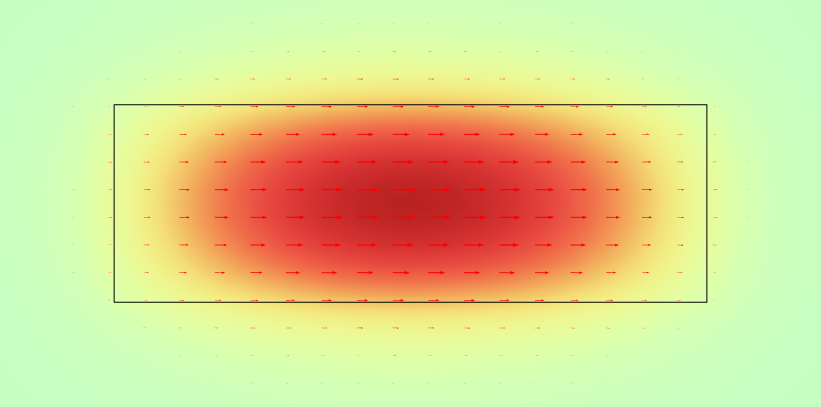
\includegraphics[scale=0.32]{SiO2_normE_1.png}
        \caption{Horizontal alignment.}
        \label{fig:E_hor}
    \end{subfigure}
    \hfill
    \begin{subfigure}{0.45\textwidth}
        \centering
        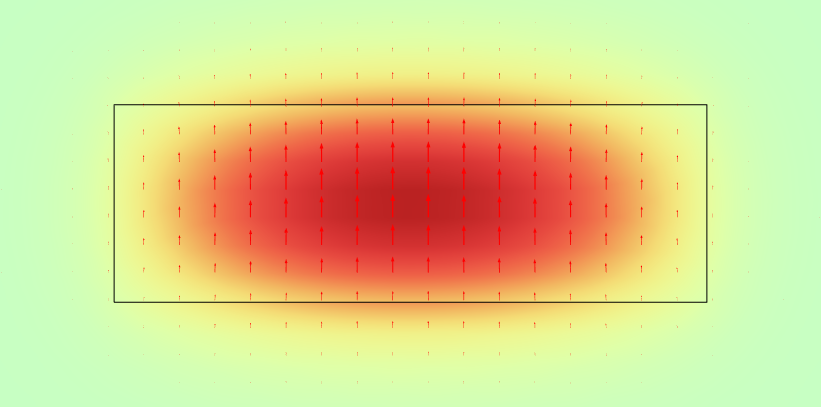
\includegraphics[scale=0.32]{SiO2_normE_2.png}
        \caption{Vertical alignment.}
        \label{fig:E_ver}
    \end{subfigure}
    \caption{Surface and arrow plots for the first two modes of the $SiO_2$ waveguide.}
\end{figure}

Different spatial distribution was also observed for higer-order modes like in the third and fifth solutions displayed in Fig. \ref{fig:third_sol} and \ref{fig:fifth_sol}, respectively.

\begin{figure}[H]
    \centering
    \begin{subfigure}{0.45\textwidth}
        \centering
        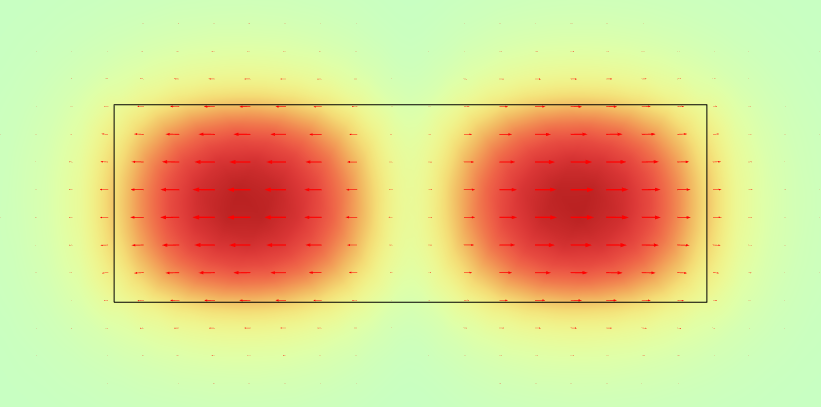
\includegraphics[scale=0.32]{SiO2_normE_3.png}
        \caption{Horizontal alignment.}
        \label{fig:third_sol}
    \end{subfigure}
    \hfill
    \begin{subfigure}{0.45\textwidth}
        \centering
        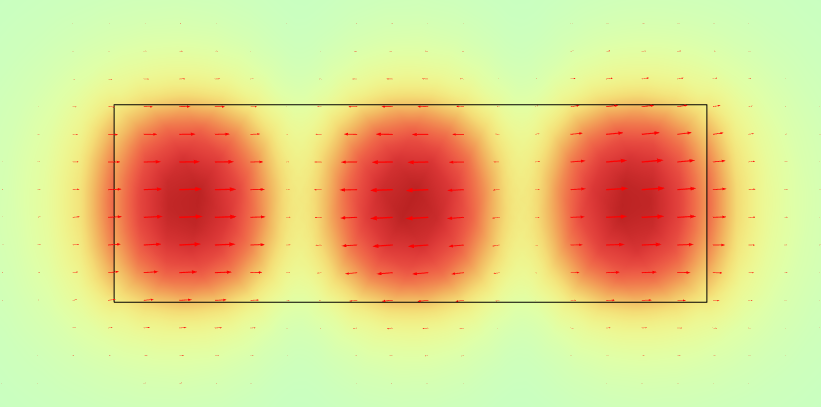
\includegraphics[scale=0.32]{SiO2_normE_5.png}
        \caption{Vertical alignment.}
        \label{fig:fifth_sol}
    \end{subfigure}
    \caption{Surface and arrow plots for the E-field for the third and fifth solutions of the $SiO_2$ waveguide.}
\end{figure}

Using the relations in Eq. \ref{eq:traverse_z}, I could generate the surface and arrow plot for the H-field. 

\begin{subequations}
    \begin{align}
        H_x = \frac{1}{i \omega \mu} \left( \frac{dE_z}{dy} - \frac{dE_y}{dz}  \right)
    \end{align}
    \begin{align}
        H_y = \frac{1}{i \omega \mu} \left( \frac{dE_x}{dz} - \frac{dE_z}{dx}  \right)
    \end{align}
    \begin{align}
        H_z = \frac{1}{i \omega \mu} \left( \frac{dE_y}{dx} - \frac{dE_x}{dy}  \right)
    \end{align}
    \label{eq:traverse_z}
\end{subequations}

The first two solutions are shown in Fig. \ref{fig:H_field}. As you can see, the H-field present a spatial distribution very different than the electric field.
            
\begin{figure}[H]
    \centering
    \begin{subfigure}{0.45\textwidth}
        \centering
        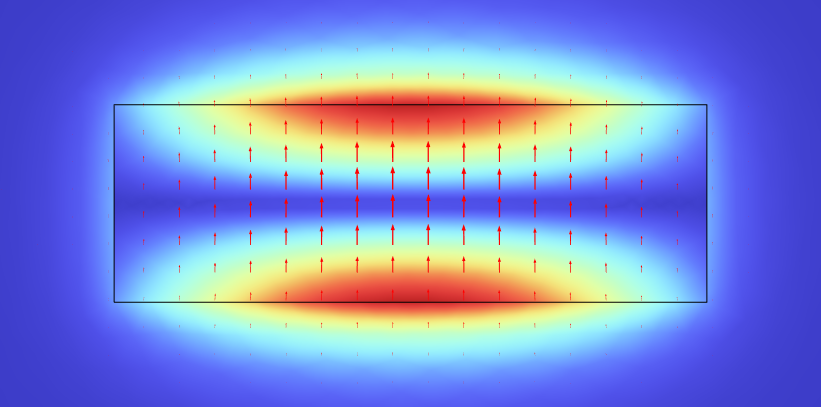
\includegraphics[scale=0.32]{SiO2_normH_1.png}
        \caption{First solution.}
    \end{subfigure}
    \hfill
    \begin{subfigure}{0.45\textwidth}
        \centering
        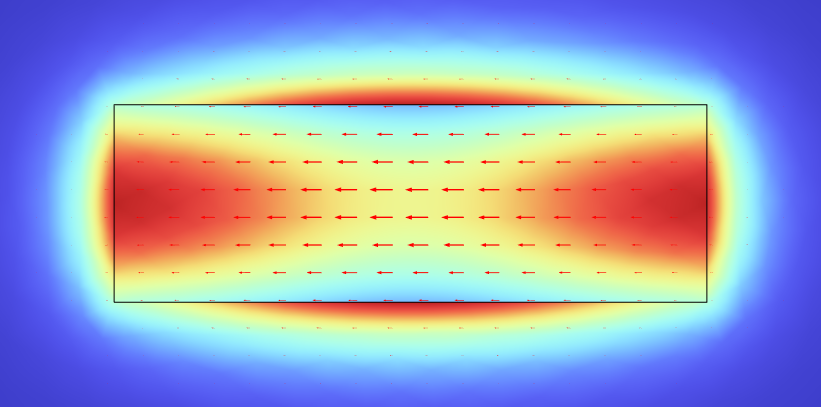
\includegraphics[scale=0.32]{SiO2_normH_2.png}
        \caption{Second solution.}
    \end{subfigure}
    \caption{Surface and arrow plots for the H-field for the first two solutions of the $SiO_2$ waveguide.}
    \label{fig:H_field}
\end{figure}

These modes COMSOL found, are they TE or TM modes? Or even, are they hybrid modes (EH/HE)? To answer this, let's analyse the average of the electrical and H-field components for each modal solution considering just the core region.

\begin{table}[H]
    \centering
    \begin{subtable}{0.45\textwidth}
        \centering
        \begin{tabular}{cccc}
            \toprule
            Solution & $\overline{E}_x$ & $\overline{E}_y$ & $\overline{E}_z$ \\
            \midrule
            1 & 35.6220 & 0.11970 & 3.1307 \\
            2 & 0.19101 & 15.9590 & 2.7269 \\
            3 & 17.6090 & 0.12490 & 3.1633 \\
            4 & 0.39748 & 15.6620 & 2.6364 \\
            5 & 11.5400 & 0.17708 & 3.2134 \\
            6 & 0.68953 & 15.5830 & 2.5424 \\
            \bottomrule
        \end{tabular}
        \caption{Electric field. The components are in $V/m$.}
    \end{subtable}
    \hfill
    \begin{subtable}{0.45\textwidth}
        \centering
        \begin{tabular}{cccc}
            \toprule
            Solution & $\overline{H}_x$ & $\overline{H}_y$ & $\overline{H}_z$ \\
            \midrule
            1 & 1.3620 & 1.1206 & 15.6140 \\
            2 & 3.1532 & 0.66509 & 4.1252 \\
            3 & 1.3802 & 2.2463 & 7.7342 \\
            4 & 3.0498 & 1.3204 & 8.2683 \\
            5 & 1.4181 & 3.3555 & 5.0526 \\
            6 & 2.9503 & 1.9693 & 12.6490 \\
            \bottomrule
        \end{tabular}
        \caption{H-field. The components are in $[\cdot 10^{-3} H/m]$.}
    \end{subtable}
    \caption{Numerical values of propagation constant and effective refractive index for the first 6 modes obtained with COMSOL for the $SiO_2$ and $TiO_2$ waveguides.}
    \label{tab:beta_num}
\end{table}

As you can see by the tables above, the z-component of the electric and H-field are comparable to the x and y components, so the mode I found are hybrid modes of the type HE ($E_z > H_z$).

Now consider the following parameters for the second simulation:
\begin{itemize}
    \item Core material: $TiO_2$.
    \item Dispersion relation: Eq. \eqref{eq:tio2_func}.
    \item Relative permeability: 1.
    \item Electric condutivity: $\sigma = 1 \cdot 10^{12}S/m$.
\end{itemize}

Afterwards, I placed the results for $\beta$ and $n_{eff}$ obtained for the $SiO_2$ and $TiO_2$ waveguides in Tab. \ref{tab:beta_num}. As you can see, for the same solution number, the modes for the $TiO_2$ case present higher value of $\beta$, confining more the light within the core when compared to the $SiO_2$ waveguide.  

\begin{table}[H]
    \centering
    \begin{subtable}{0.45\textwidth}
        \centering
        \begin{tabular}{ccc}
            \toprule
            Solution & $\beta [\mu m^{-1}]$ & $n_{eff}$ \\
            \midrule
            1 & 4.555 & 1.124 \\
            2 & 4.536 & 1.119 \\
            3 & 4.482 & 1.106 \\
            4 & 4.468 & 1.102 \\
            5 & 4.361 & 1.076 \\
            6 & 4.353 & 1.074 \\
            \bottomrule
        \end{tabular}
        \caption{$SiO_2$.}
    \end{subtable}
    \hfill
    \begin{subtable}{0.45\textwidth}
        \centering
        \begin{tabular}{ccc}
            \toprule
            Mode & $\beta [\mu m^{-1}]$ & $n_{eff}$ \\
            \midrule
            1 & 6.005 & 1.482 \\
            2 & 6.024 & 1.486 \\
            3 & 6.104 & 1.506 \\
            4 & 6.130 & 1.512 \\
            5 & 6.163 & 1.520 \\
            5 & 6.193 & 1.528 \\
            \bottomrule
        \end{tabular}
        \caption{$TiO_2$.}
    \end{subtable}
    \caption{Numerical values of propagation constant and effective refractive index for the first 6 modes obtained with COMSOL for the $SiO_2$ and $TiO_2$ waveguides.}
    \label{tab:beta_num}
\end{table}

The modes found in this section don't agree with the TE modes we calculated in Sec. \ref{subsec:rectangular_dielectric_waveguide}, where we used the variable separation approximation. Since the solver of COMSOL don't use this approximation, it simply solves the eigenvalue equation Eq. \ref{eq:eigen} using a numerical method, COMSOL is to be trusted.

\begin{equation}
    \nabla \times \left( \frac{1}{\mu_r} \nabla \times \mathbf{E} \right) = k_0^2 \epsilon_r \mathbf{E}
    \label{eq:eigen}
\end{equation}

\subsection{Coupled guides}
\label{subsec:coupled_guides}

Now, let's consider a waveguide made by an air cladding and two equal cores. The geometrical parameters of the simulations are as follow:
\begin{itemize}
    \item Cladding:
    \begin{itemize}
        \item $w = 30\mu m$.
        \item $t = 15\mu m$.
    \end{itemize}
    \item Core 1 and 2:
    \begin{itemize}
        \item $w = 6\mu m$.
        \item $t = 2\mu m$. 
    \end{itemize}
\end{itemize}

Varying the gap distance $d$ between the cores for the $SiO_2/SiO_2$ waveguide, we get the plots of Fig. \ref{fig:varying_d}. You can see that at $d = 1\mu m$, the modes of the different cores almost don't perceive the modes of the adjascent core. As you decrease the gap between them, the system tends to converge to one waveguide at $d = 0\mu m$ with $w = w_{core1} + w_{core} = 12\mu m$ and $t = 2\mu m$.

\begin{figure}[H]
    \centering
    \begin{subfigure}{0.45\textwidth}
        \centering
        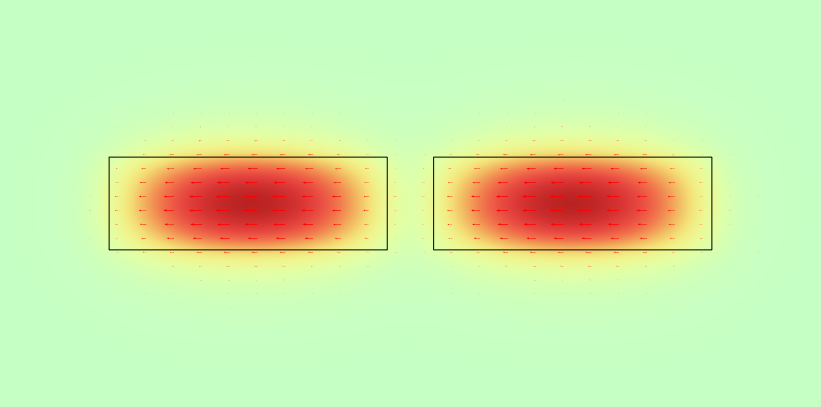
\includegraphics[scale=0.32]{SiO2_SiO2_normE_0_d1um.png}
        \caption{$d = 1\mu m$.}
    \end{subfigure}
    \hfill
    \begin{subfigure}{0.45\textwidth}
        \centering
        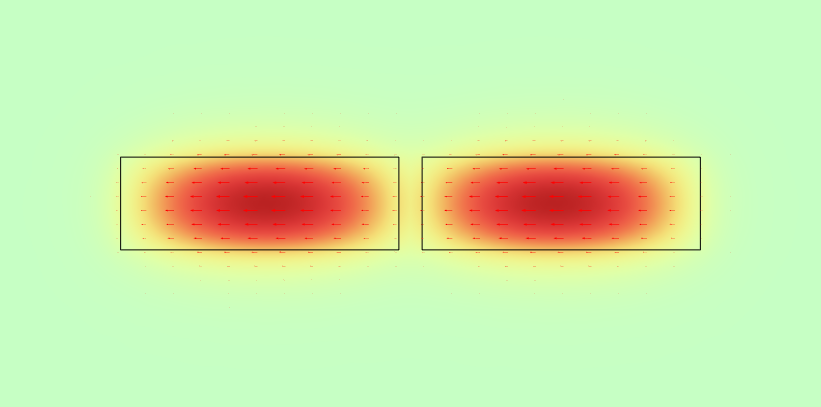
\includegraphics[scale=0.32]{SiO2_SiO2_normE_0_d0.5um.png}
        \caption{$d = 0.5\mu m$.}
    \end{subfigure}
    \hfill
    \begin{subfigure}{0.45\textwidth}
        \centering
        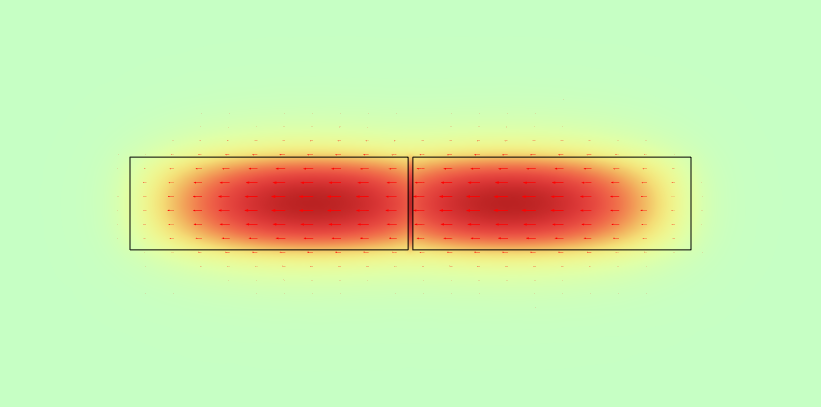
\includegraphics[scale=0.32]{SiO2_SiO2_normE_0_d0.1um.png}
        \caption{$d = 0.1\mu m$.}
    \end{subfigure}
    \hfill
    \begin{subfigure}{0.45\textwidth}
        \centering
        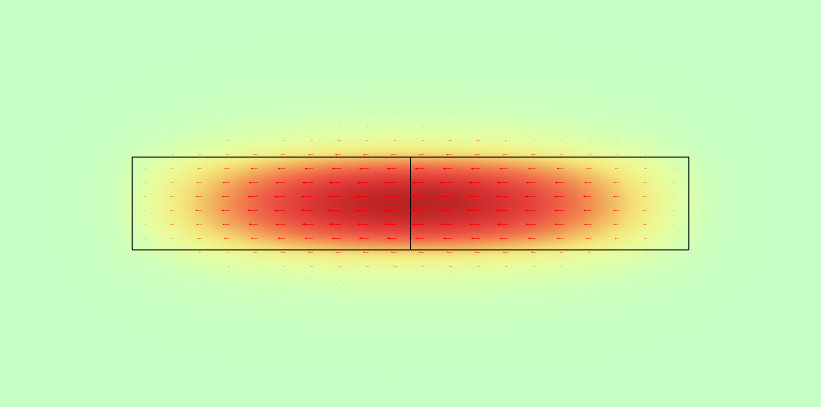
\includegraphics[scale=0.32]{SiO2_SiO2_normE_0_d0um.png}
        \caption{$d = 0\mu m$.}
    \end{subfigure}
    \caption{Surface and arrow plots for the E-field for the first solution of the $SiO_2/SiO_2$ coupled waveguide for different gaps $d$.}
    \label{fig:varying_d}
\end{figure}

To explore the high confinement of the $TiO_2$, we solved the problem for $SiO_2/SiO_2$ and $TiO_2/TiO_2$ waveguides for $d = 0.5\mu m$. As expected, the overlaping region for the $TiO_2/TiO_2$ guide is smaller for the fundamental mode. Something more interesting happens when we consider the core of different materials, the $SiO_2/TiO_2$. Only the core of $TiO_2$ guides light.

\begin{figure}[H]
    \centering
    \begin{subfigure}{0.45\textwidth}
        \centering
        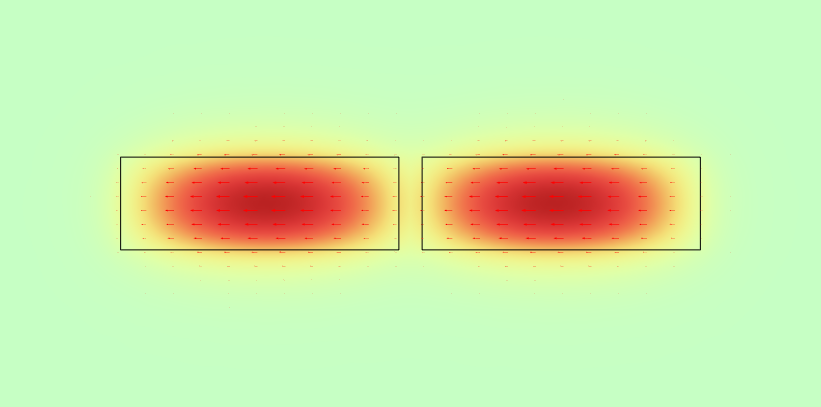
\includegraphics[scale=0.32]{SiO2_SiO2_normE_0_d0.5um.png}
        \caption{$SiO_2/SiO_2$.}
    \end{subfigure}
    \hfill
    \begin{subfigure}{0.45\textwidth}
        \centering
        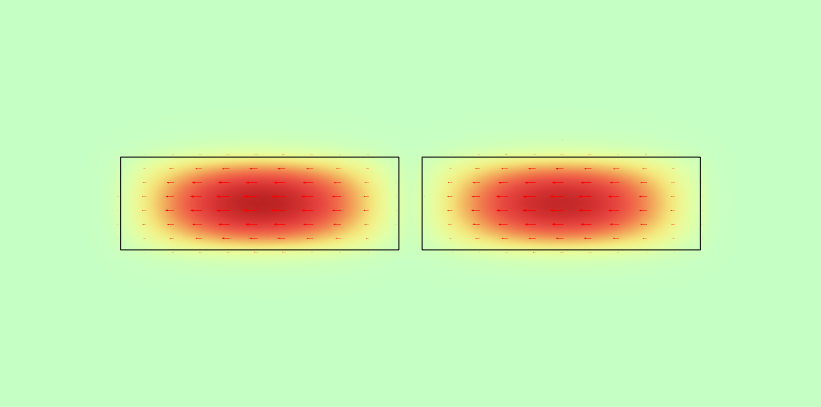
\includegraphics[scale=0.32]{TiO2_TiO2_normE_0_d0.5um.png}
        \caption{$TiO_2/TiO_2$.}
    \end{subfigure}
    \hfill
    \begin{subfigure}{0.45\textwidth}
        \centering
        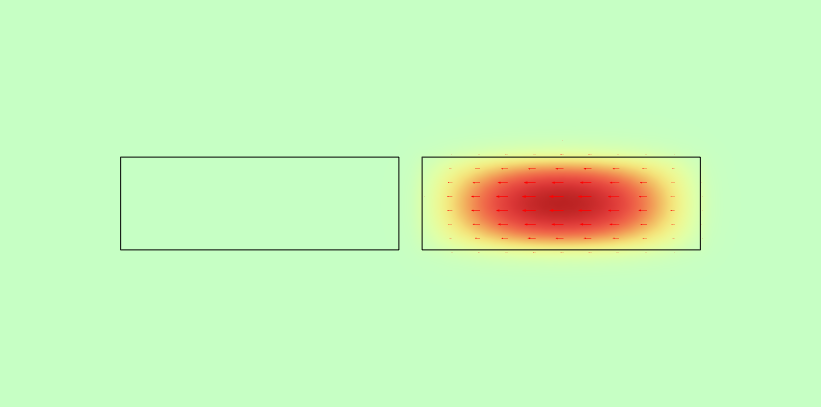
\includegraphics[scale=0.32]{SiO2_TiO2_normE_0_d0.5um.png}
        \caption{$SiO_2/TiO_2$.}
    \end{subfigure}
    \caption{Comparison between the waveguides $SiO_2/SiO_2$, $TiO_2/TiO_2$, and $SiO_2/TiO_2$ for $d = 0.5\mu m$.}
    \label{fig:different_mat_cores}
\end{figure}

Now, let's explore the impact of varying the shape of the 
second core. Let's double it, so $w_{core2} = 12\mu m$ and $t_{core2} = 4 \mu m$, but with the center of the cores being aligned. The results are shown in Fig. \ref{fig:double_size}.

\begin{figure}[H]
    \centering
    \begin{subfigure}{0.45\textwidth}
        \centering
        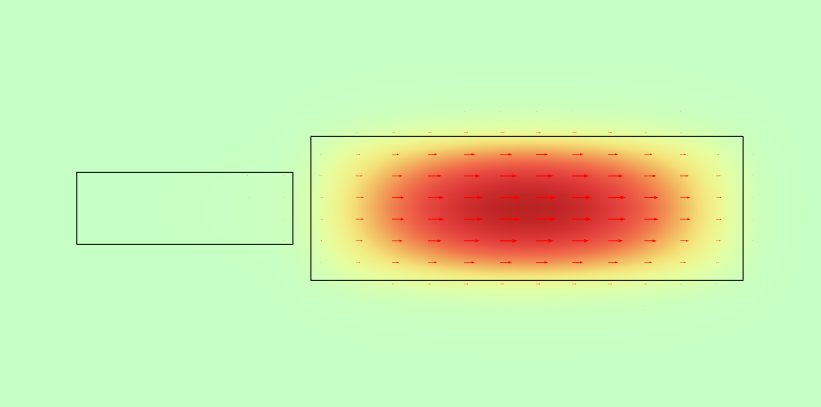
\includegraphics[scale=0.32]{SiO2_SiO2_d0.5um_w12um_t4um_normE_0.png}
        \caption{First solution.}
    \end{subfigure}
    \hfill
    \begin{subfigure}{0.45\textwidth}
        \centering
        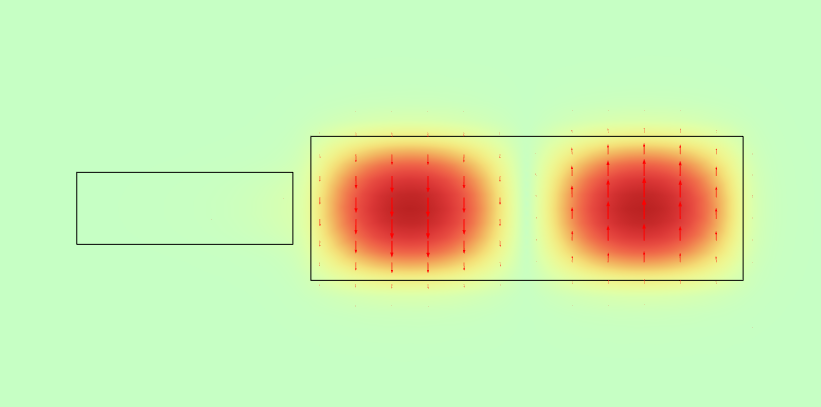
\includegraphics[scale=0.32]{SiO2_SiO2_d0.5um_w12um_t4um_normE_3.png}
        \caption{Fourth solution.}
    \end{subfigure}
    \hfill
    \begin{subfigure}{0.45\textwidth}
        \centering
        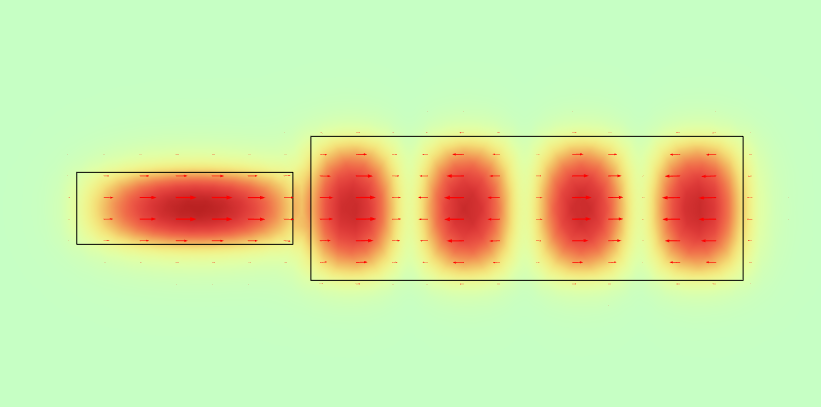
\includegraphics[scale=0.32]{SiO2_SiO2_d0.5um_w12um_t4um_normE_6.png}
        \caption{Seventh solution.}
    \end{subfigure}
    \hfill
    \begin{subfigure}{0.45\textwidth}
        \centering
        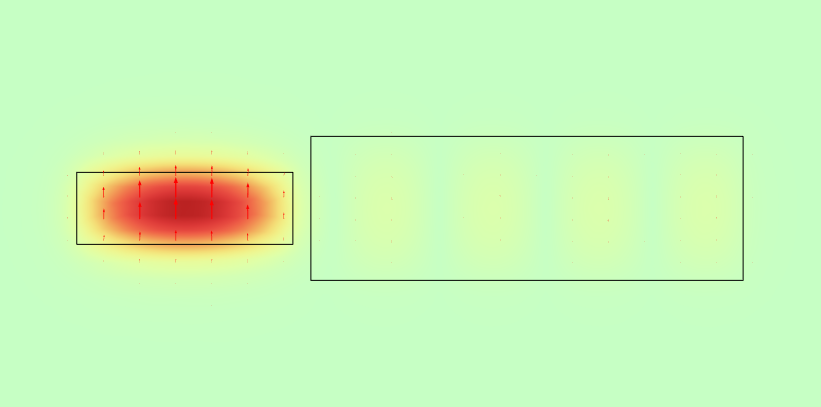
\includegraphics[scale=0.32]{SiO2_SiO2_d0.5um_w12um_t4um_normE_9.png}
        \caption{Tenth solution.}
    \end{subfigure}
    \caption{Solution of the supermodes for the $SiO_2/SiO_2$ waveguide with the second core with doubled dimensions.}
    \label{fig:double_size}
\end{figure}

As you can see, for the first supermodes, they are confined majoritaly in the larger core. As we increase the number of modes, starts to appear some supermodes guided through both cores. If we keep increasing the oreder of the solution, it will arise supermodes majoritaly guided through the smaller core. 

If we return to the case of two cores with identical shapes for the $SiO_2/SiO_2$ coupled waveguide and shift the position of the right-side core breaking the symmetry, what does happen? The shift in the y-direction acts like a gap and change the shape of the overlapping region as you can see in Fig. \ref{fig:shifted_core2}.

\begin{figure}[H]
    \centering
    \begin{subfigure}{0.45\textwidth}
        \centering
        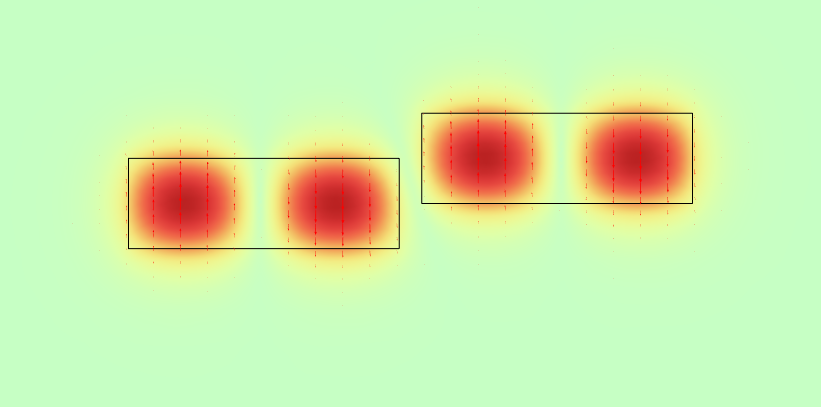
\includegraphics[scale=0.32]{SiO2_SiO2d_0.5um_dy1um_normE_7.png}
        \caption{Eigth solution.}
    \end{subfigure}
    \hfill
    \begin{subfigure}{0.45\textwidth}
        \centering
        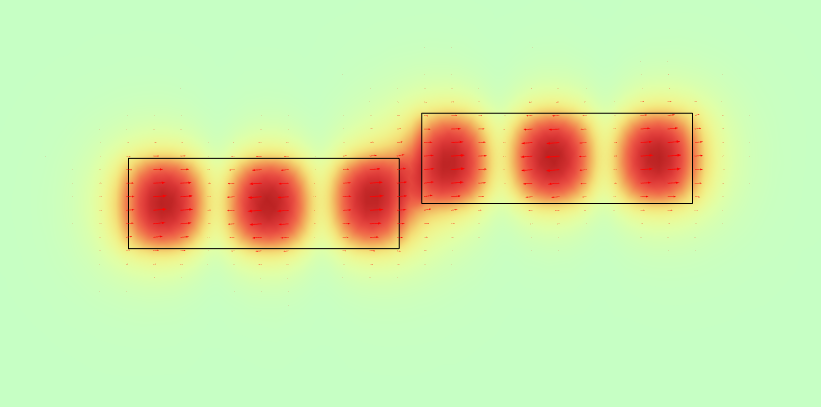
\includegraphics[scale=0.32]{SiO2_SiO2d_0.5um_dy1um_normE_8.png}
        \caption{Nineth solution.}
    \end{subfigure}
    \caption{Even and odd supermodes of the coupled waveguide $SiO_2/SiO_2$.}
    \label{fig:shifted_core2}
\end{figure}


Furthermore, it is very important to understand that COMSOL solves for the supermodes of the coupled waveguide in the modal analysis, returning even and odd modes. You can see the even supermode in Fig. \ref{fig:even_supermode} where the transverse electric field is in the same direction in both cores, and the odd supermode are characterized by the oposite direction of this electric field in the different cores and is shown in Fig. \ref{fig:odd_supermode}.

\begin{figure}[H]
    \centering
    \begin{subfigure}{0.45\textwidth}
        \centering
        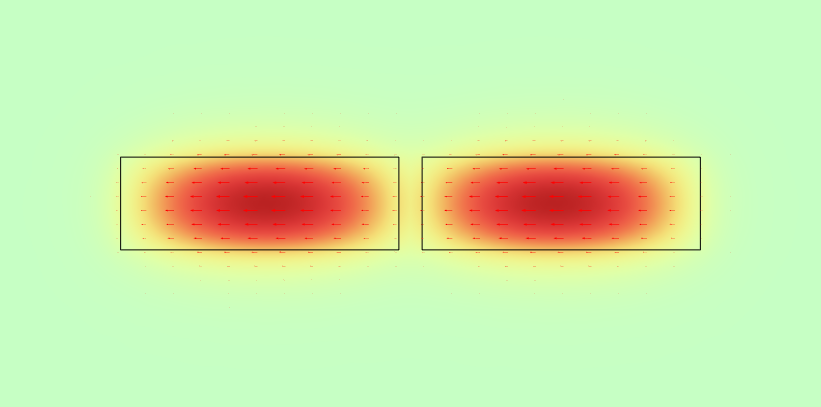
\includegraphics[scale=0.32]{SiO2_SiO2_normE_0_d0.5um.png}
        \caption{Even.}
        \label{fig:even_supermode}
    \end{subfigure}
    \hfill
    \begin{subfigure}{0.45\textwidth}
        \centering
        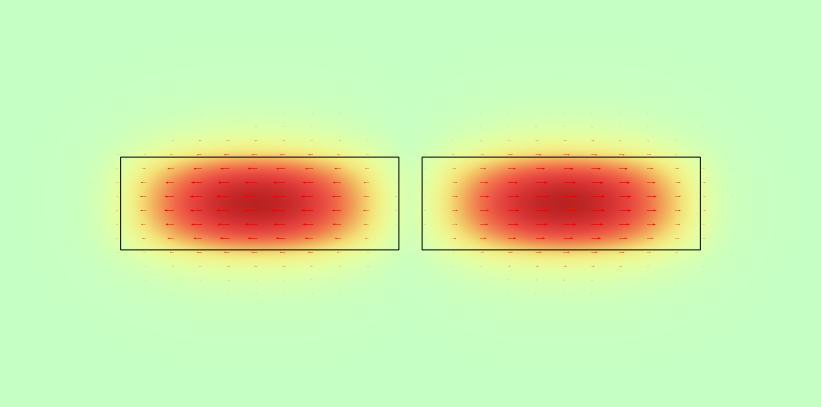
\includegraphics[scale=0.32]{SiO2_SiO2_normE_1_d0.5um.png}
        \caption{Odd.}
        \label{fig:odd_supermode}
    \end{subfigure}
    \caption{Even and odd supermodes of the coupled waveguide $SiO_2/SiO_2$.}
\end{figure}

From the mode analyse we obtain $n_{eff}$ of the supermodes, making it possible to calculate $\beta = k_0 n_{eff}$. By identifying the even and odd modes in $\{\beta_{even,j}\}_j$ and $\{\beta_{odd,j}\}_j$, respectively, we can calculate the coupling length $L_{c,j}$, the parameter that says what is the necessary length for the j-th supermode to be completely coupled from the first core to the second core. It is given by Eq. \eqref{eq:coupling_length}.

\begin{equation}
    L_{c,j} = \frac{\pi}{|\Delta \beta_j|}, \quad \Delta \beta_j = \beta_{even, j} - \beta_{odd, j} 
    \label{eq:coupling_length}
\end{equation}

To help in the task of calculating $L_{c,j}$, I put in Tab. \ref{tab:coupling_length_aux} the values of the order of the supermode, effective refractive index and propagation constant by separating the even from the odd supermodes.

\begin{table}[H]
    \centering
    \begin{subtable}{0.45\textwidth}
        \centering
        \begin{tabular}{ccc}
            \toprule
            Order & $n_{eff}$ & $\beta [\mu m^{-1}]$ \\
            \midrule
            0 & 1.1241 & 4.557 \\
            1 & 1.1197 & 4.539 \\
            2 & 1.1043 & 4.476 \\
            3 & 1.1006 & 4.461 \\
            \bottomrule
        \end{tabular}
        \caption{Even.}
    \end{subtable}
    \hfill
    \begin{subtable}{0.45\textwidth}
        \centering
        \begin{tabular}{ccc}
            \toprule
            Order & $n_{eff}$ & $\beta [\mu m^{-1}]$ \\
            \midrule
            0 & 1.1233 & 4.553 \\
            1 & 1.1187 & 4.535 \\
            2 & 1.1077 & 4.490 \\
            3 & 1.1044 & 4.477 \\
            \bottomrule
        \end{tabular}
        \caption{Odd.}
    \end{subtable}
    \caption{Auxiliary table to calculate the coupling length of supermodes.}
    \label{tab:coupling_length_aux}
\end{table}

Now, we can calculate the coupling length. Note, that if we want the second core to guide $\eta [\%]$ of the input light guided through the first core, we must have a interaction length $L_{int, j} = \eta L_{c, j}$. So, for a 50/50 beamsplitter, $L_{int, j} = L_{c,j} / 2$. The results are placed in Tab. \ref{tab:coupling_length}.

\begin{table}[H]
    \centering
    \begin{tabular}{cccc}
        \toprule
        Order & $|\Delta \beta| [\mu m^{-1}]$ & $L_c [\mu m]$ & $L_{c}/2 [\mu m]$ \\
        \midrule
        0 & 0.003 & 969 & 485 \\     
        1 & 0.004 & 775 & 388 \\
        2 & 0.014 & 228 & 114 \\
        3 & 0.015 & 204 & 102 \\
        \bottomrule
    \end{tabular}
    \caption{Coupling length for the supermodes.}
    \label{tab:coupling_length}
\end{table}

As you can infer, as we increase the order of the supermode, we increase the interaction between the cores making possible to exchange energy easier from the first core to the second core, decreasing the interaction length needed to obtain total or 50/50 coupling.

\subsection{Beamsplitter 50/50}
\label{subsec:beamsplitter}

Based on the results of the Sec. \ref{subsec:coupled_guides}, I chose to design a beamsplitter 50/50 for the $SiO_2/SiO_2$ waveguide, since $SiO_2$ present less light confinement compared to $TiO_2$ \textemdash remember we want to enhance coupling efficiency for lesser interaction lengths. Furthermore, I chose the cores to be identical in material, all $SiO_2$, to ensure one core doesn't confine more light than the other. And to simplify, we will let the cores to be aligned so there is no gap effect in the y-direction. At last, considering the difficulties involved in the fabrication of devices with less than a few hundred of nanometers, I will take the gap to be $d = 0.5\mu m = 500nm$.

For the first study, consider the cores to present the same geometrical parameters: $w_{core, j} = 6\mu m$ and $t_{core, j} = 2\mu m$. Also, consider the input light entering at the first core only at the beginning ($P_{z,2}(0) = 0$) with $\lambda = 1.55\mu m = 1550nm$. Since in most applications the fundamental mode is the desired one, let's consider just it, so just the first supermode.

To help to calculate the coupling length for the first supermode, I created the Tab. \ref{tab:wv_var_aux}.

\begin{table}[H]
    \centering
    \begin{subtable}{0.45\textwidth}
        \centering
        \begin{tabular}{ccc}
            \toprule
            $\lambda [\mu m]$ & $n_{eff}$ & $\beta [\mu m^{-1}]$ \\
            \midrule
            1.40 & 1.1394 & 5.1136 \\
            1.45 & 1.1345 & 4.9161 \\
            1.50 & 1.1295 & 4.7312 \\
            1.55 & 1.1241 & 4.5567 \\
            1.60 & 1.1185 & 4.3923 \\
            1.65 & 1.1126 & 4.2368 \\
            1.70 & 1.1064 & 4.0892 \\
            \bottomrule
        \end{tabular}
        \caption{Even.}
    \end{subtable}
    \hfill
    \begin{subtable}{0.45\textwidth}
        \centering
        \begin{tabular}{ccc}
            \toprule
            $\lambda [\mu m]$ & $n_{eff}$ & $\beta [\mu m^{-1}]$ \\
            \midrule
            1.40 & 1.1389 & 5.1114 \\
            1.45 & 1.1340 & 4.9139 \\
            1.50 & 1.1288 & 4.7283 \\
            1.55 & 1.1233 & 4.5535 \\
            1.60 & 1.1176 & 4.3649 \\
            1.65 & 1.1115 & 4.2326 \\
            1.70 & 1.1051 & 4.0844 \\
            \bottomrule
        \end{tabular}
        \caption{Odd.}
    \end{subtable}
    \caption{Auxiliary table to calculate the coupling length of the first supermode varying the input wavelength for the identical cores.}
    \label{tab:wv_var_aux}
\end{table}

The coupling length for the different wavelengths was computed and placed in Tab. \ref{tab:wv_var}.

\begin{table}[H]
    \centering
    \begin{tabular}{ccc}
        \toprule
        $\lambda [\mu m]$ & $L_c$ & $\eta[\%]$ \\
        \midrule
        1.40 & 1400.0 & 34.6 \\
        1.45 & 1450.0 & 33.4 \\
        1.50 & 1071.4 & 45.2 \\
        1.55 & 968.7 & 50.0 \\
        1.60 & 888.9 & 54.5 \\
        1.65 & 750.0 & 64.59 \\
        1.70 & 653.8 & 74.09 \\    
        \bottomrule
    \end{tabular}
    \caption{Coupling length and coupling efficiency coefficient for the first supermode making $L_{int} = 484.4\mu m$ varying the input wavelength for the identical cores.}
    \label{tab:wv_var}
\end{table}

As you can see, this coupled waveguide works well as a 50/50 splitter within the error $\pm 5$ in the range $\lambda \in [1.50 \mu m, 1.60\mu m]$. 

Now, consider the following dimensions: $w_{core1} = 3\mu m$, $w_{core2} = 6\mu m$ and $t_{core,j} = 2\mu m$.

\begin{table}[H]
    \centering
    \begin{subtable}{0.45\textwidth}
        \centering
        \begin{tabular}{ccc}
            \toprule
            $\lambda [\mu m]$ & $n_{eff}$ & $\beta [\mu m^{-1}]$ \\
            \midrule
            1.40 & 1.1392 & 5.1127 \\
            1.45 & 1.1343 & 4.9152 \\
            1.50 & 1.1291 & 4.7296 \\
            1.55 & 1.1237 & 4.5551 \\
            1.60 & 1.1181 & 4.3908 \\
            1.65 & 1.1121 & 4.2349 \\
            1.70 & 1.1058 & 4.0870 \\
            \bottomrule
        \end{tabular}
        \caption{Even.}
    \end{subtable}
    \hfill
    \begin{subtable}{0.45\textwidth}
        \centering
        \begin{tabular}{ccc}
            \toprule
            $\lambda [\mu m]$ & $n_{eff}$ & $\beta [\mu m^{-1}]$ \\
            \midrule
            1.40 & 1.1353 & 5.0952 \\
            1.45 & 1.1302 & 4.8974 \\
            1.50 & 1.1248 & 4.7116 \\
            1.55 & 1.1193 & 4.5373 \\
            1.60 & 1.1134 & 4.3723 \\
            1.65 & 1.1074 & 4.2170 \\
            1.70 & 1.1010 & 4.0693 \\
            \bottomrule
        \end{tabular}
        \caption{Odd.}
    \end{subtable}
    \caption{Auxiliary table to calculate the coupling length of the first supermode varying the input wavelength for different size cores.}
    \label{tab:wv_var_aux_doub}
\end{table}

\begin{table}[H]
    \centering
    \begin{tabular}{ccc}
        \toprule
        $\lambda [\mu m]$ & $L_c$ & $\eta[\%]$ \\
        \midrule
        1.40 & 179.5 & 49.1 \\
        1.45 & 176.8 & 49.8 \\
        1.50 & 174.4 & 50.5 \\
        1.55 & 176.1 & 50.0 \\
        1.60 & 170.2 & 51.8 \\
        1.65 & 175.5 & 50.2 \\
        1.70 & 177.1 & 49.7 \\    
        \bottomrule
    \end{tabular}
    \caption{Coupling length and coupling efficiency coefficient for the first supermode making $L_{int} = 88.1\mu m$ varying the input wavelength for different size cores.}
    \label{tab:wv_var}
\end{table}

Surprinsingly, this resulted in a more robust 50/50 within $\pm 2\%$ in the range $\lambda \in [1.40 \mu m, 1.70\mu]$. If we accept a margin of $\pm 10\%$ we can extand this range even further. 

\end{document}